\documentclass[conference]{IEEEtran}
\usepackage{amsmath, amssymb, graphicx, cite, hyperref}
\usepackage{tikz}
\usetikzlibrary{calc,arrows.meta,positioning,fit,shapes.geometric}

% ---------- Title ----------
\title{SkyEdge: Secure High-Altitude Drone Platform Integrating $H_\infty$ Control, Domestic Devices, and Advanced Mechanical Design}

% ---------- Author ----------
\author{
\IEEEauthorblockN{Shinichi Samizo}
\IEEEauthorblockA{Independent Semiconductor Researcher \\
Project Design Hub, Samizo-AITL \\
\textit{Email:} \href{mailto:shin3t72@gmail.com}{shin3t72@gmail.com} \\
\textit{GitHub:} \href{https://github.com/Samizo-AITL}{Samizo-AITL}}
}

\begin{document}
\maketitle

% ---------- Abstract ----------
\begin{abstract}
This paper presents the foundational design of \emph{SkyEdge}, 
a secure high-altitude unmanned aerial vehicle (UAV) platform that 
integrates $H_\infty$ control, domestic devices, and a variable-pitch 
mechanical structure. The proposed framework provides robust disturbance 
rejection, secure hardware implementation, and reliable flight capability 
up to 10,000 m altitude. We describe the control architecture, device 
integration, and mechanical design, and we outline evaluation plans 
toward a proof-of-concept prototype.
\end{abstract}

% ---------- Keywords ----------
\begin{IEEEkeywords}
UAV, robust control, $H_\infty$, variable-pitch rotor, secure systems, high-altitude flight
\end{IEEEkeywords}

% ---------- Sections ----------
\section{Introduction}
Unmanned aerial vehicles (UAVs) are increasingly important in defense, 
disaster response, and environmental monitoring. However, most commercial 
systems are limited to altitudes below 3,000 m, and many rely on 
foreign-made devices with security concerns. This paper aims to establish 
a domestic, secure UAV platform capable of robust operation in 
high-altitude environments.

\section{Related Work}
Control approaches such as PID, adaptive control, and sliding-mode 
control have been applied to UAVs, but robust performance under strong 
disturbances remains challenging. $H_\infty$ control has potential for 
disturbance rejection. Existing high-altitude UAV programs (NASA Helios, 
JAXA HAPS) demonstrate feasibility but rely on specialized designs. 
Security aspects and domestic device integration remain underexplored.

\section{System Architecture}
The proposed architecture integrates three layers:
\begin{itemize}
    \item \textbf{$H_\infty$ Control:} ensures robustness against gusts 
    up to 20--30 m/s.
    \item \textbf{FSM:} manages mode transitions (normal, high-altitude, 
    comm-loss, emergency return).
    \item \textbf{LLM:} assists adaptive redesign of control policies in 
    unforeseen conditions (simulation environment).
\end{itemize}

\begin{figure}[t]
\centering
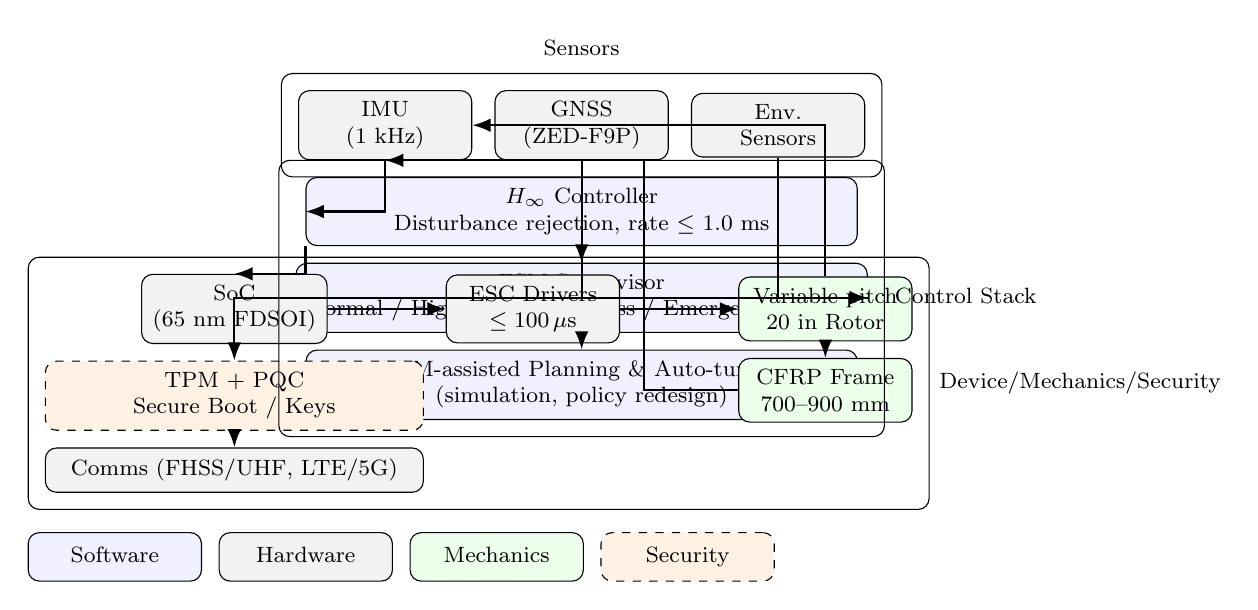
\begin{tikzpicture}[
    font=\footnotesize,
    node distance=6pt and 8pt,
    box/.style={draw, rounded corners, align=center, inner sep=4pt, minimum width=2.2cm},
    hw/.style={box, fill=gray!10},
    sw/.style={box, fill=blue!6},
    mech/.style={box, fill=green!8},
    sec/.style={box, fill=orange!10, dashed},
    arrow/.style={-Latex, thick},
    grp/.style={draw, rounded corners, inner sep=6pt}
]

% ===== Sensors / Environment =====
\node[hw] (imu) {IMU\\(1 kHz)};
\node[hw, right=of imu] (gps) {GNSS\\(ZED-F9P)};
\node[hw, right=of gps] (env) {Env.\\Sensors};

% ===== H-infty control (inner loop) =====
\node[sw, below=of gps, minimum width=7.0cm] (hinf) {$H_\infty$ Controller\\
Disturbance rejection, rate $\leq$ 1.0 ms};

% ===== FSM (supervisory) =====
\node[sw, below=of hinf, minimum width=7.0cm] (fsm) {FSM Supervisor\\
Normal / High-alt / Comm-loss / Emergency Return};

% ===== LLM planning (outer loop) =====
\node[sw, below=of fsm, minimum width=7.0cm] (llm) {LLM-assisted Planning \& Auto-tuning\\
(simulation, policy redesign)};

% ===== Hardware stack =====
\node[hw, below left=10pt and -8pt of hinf] (soc) {SoC\\(65 nm FDSOI)};
\node[hw, right=1.5cm of soc] (esc) {ESC Drivers\\$\leq 100\,\mu$s};
\node[mech, right=1.5cm of esc] (vp) {Variable-pitch\\20 in Rotor};
\node[mech, below=of vp] (frame) {CFRP Frame\\700--900 mm};
\node[sec, below=of soc, minimum width=4.8cm] (secblk) {TPM + PQC\\Secure Boot / Keys};
\node[hw, below=of secblk, minimum width=4.8cm] (comms) {Comms (FHSS/UHF, LTE/5G)};

% ===== Group boxes =====
\node[grp, fit=(imu)(gps)(env), label=above:{\strut Sensors}] (gSensors) {};
\node[grp, fit=(hinf)(fsm)(llm), label=right:{\strut Control Stack}] (gCtrl) {};
\node[grp, fit=(soc)(esc)(vp)(frame)(secblk)(comms), 
      label=right:{\strut Device/Mechanics/Security}] (gHW) {};

% ===== Connections =====
\draw[arrow] (imu.south) |- (hinf.west);
\draw[arrow] (gps.south) |- (fsm.east);
\draw[arrow] (env.south) |- (fsm.east);

\draw[arrow] (hinf.south) -- (fsm.north);
\draw[arrow] (fsm.south) -- (llm.north);

\draw[arrow] (hinf.south west) |- (soc.north);
\draw[arrow] (soc.east) -- (esc.west);
\draw[arrow] (esc.east) -- (vp.west);
\draw[arrow] (vp.south) -- (frame.north);

\draw[arrow] (fsm.east) -| (secblk.north);
\draw[arrow] (secblk.south) -- (comms.north);

% Feedback from sensors to control stack
\draw[arrow] (frame.west) -| ++(-1.2,0) |- (imu.south);
\draw[arrow] (vp.north) |- (imu.east);

% ===== Legend (fixed) =====
\node[box, fill=blue!6, anchor=north west] (lg1)
      at ($(gHW.south west)+(0,-8pt)$) {\strut Software};
\node[box, fill=gray!10, anchor=north west, right=6pt of lg1] (lg2)
      {\strut Hardware};
\node[box, fill=green!8, anchor=north west, right=6pt of lg2] (lg3)
      {\strut Mechanics};
\node[box, fill=orange!10, dashed, anchor=north west, right=6pt of lg3] (lg4)
      {\strut Security};

\end{tikzpicture}
\caption{SkyEdge system architecture: three-layer control stack ($H_\infty$, FSM, LLM) integrated with sensors, secure device stack (SoC, TPM/PQC, comms), and variable-pitch mechanical design.}
\label{fig:sysarch}
\end{figure}

\section{Device Integration}
The device layer includes a domestic SoC (65 nm FDSOI), LDMOS motor 
drivers, high-rate IMU (1 kHz), and secure modules (TPM + PQC). 
Control cycle is maintained at $\leq 1.0$ ms with ESC response $\leq 100 
\, \mu$s. Estimated BOM cost is 596,700 JPY per unit (with reduction in 
mass production).

\section{Mechanical Design}
The UAV has a 700--900 mm frame, CFRP structure, and a variable-pitch 
20-inch rotor system. At take-off weight 6.38 kg, the thrust-to-weight 
ratio is $\approx 2.82$. Variable pitch enables adaptation from sea 
level to 10,000 m (RPM from $\approx 8,339$ to $14,353$). Servo torque 
requirement is 0.62 N$\cdot$m with safety factor of 2--3.

\section{Evaluation Plan}
Planned evaluations include wind-tunnel testing, low-temperature chamber 
tests, redundancy verification, and communication robustness under 
jamming scenarios. A proof-of-concept schedule has been drafted for 
2025--2026.

\section{Conclusion}
We presented the SkyEdge architecture integrating $H_\infty$ control, 
domestic devices, and mechanical design for secure high-altitude UAVs. 
The proposed system addresses robustness, security, and reliability at 
10,000 m operation. Future work includes prototype development and 
extension to underwater vehicles (\emph{SeaEdge}), toward a unified 
autonomous platform for defense, disaster response, GX, and education.

% ---------- References ----------
\bibliographystyle{IEEEtran}
\bibliography{refs}

\end{document}
